\section{Fourfold display for 2 x 2 tables}\label{sec:twoway-fourfold}
\ixon{fourfold display}
The \boldital{fourfold display} is a relative of the pie chart,
designed for the display of $2 \times 2$ (or $2 \times 2 \times k$)
tables
\citep{Fienberg:75,Friendly:94b,Friendly:94c}.
In this display the frequency
\(n_{ij}\) in each cell of a fourfold table is shown by a quarter
circle, whose radius is proportional to \(\sqrt { n_{ij} }\), so the
area is proportional to the cell count.
The fourfold display
is similar to a pie chart in using segments of
a circle to show frequencies.  It
differs from a pie chart in that it keeps the
angles of the segments constant and varies the radius,
whereas the pie chart varies the angles and keeps the radius constant.

The main purpose of this display is to depict the sample odds ratio,
\(\hat{\theta} = (n_{11} /  n_{12} )
\div  (n_{21} /  n_{22} )\).  An association between the variables
(\(\theta \neq 1\)) is shown by the tendency of diagonally opposite
cells in one direction to differ in size from those in the opposite
direction, and the display uses color or shading to show this
direction.  Confidence rings for the observed \(\theta\) allow a
visual test of the hypothesis of independence,
 \(H_0 :  \theta  =  1\).  They have
the property that (in a standardized display) the rings for adjacent quadrants overlap \emph{iff}
the observed counts are consistent with the null hypothesis.

\begin{Example}[berkeley2]{Berkeley admissions}
\figref{fig:fourfold11} shows the basic fourfold display for the
Berkeley admissions data (\tabref{tab:berk22}).
Here, the area of each quadrant is proportional to the cell frequency,
shown numerically in each corner.
The odds ratio is proportional to the product of the areas
shaded dark, divided by the product of the areas shaded light.
The sample odds ratio, Odds (Admit\(|\)Male) / Odds(Admit\(|\)Female) is
1.84 (see \exref{ex:berkeley1a})
indicating that males were nearly twice as likely to be admitted.

However, it is difficult to make these visual comparisons
because there are more men than women, and because the
proportions admitted and rejected are unequal.  In the unstandardized
display the confidence bands have no interpretation as a test
of \(H_0 :  \theta  =  1\).
\fig{fourfold11}{scale=.6}{Fourfold display for Berkeley admission data, unstandardized}


The data in a $2 \times 2$ table can be standardized to make these
visual comparisons easier.
\tabref{tab:berkrow} shows the Berkeley data with the addition of
row percentages (which equate for the number of men and women applicants)
 indicating the proportion of each gender accepted
and rejected.
We see that 44.52\% of males were admitted, while only 30.35\% of
females were admitted.
Moreover, the row percentages have the same odds ratio as the
raw data: $44.52 \times 69.65 / 30.35 \times 55.48 = 1.84$.
\figref{fig:fourfold12} shows the fourfold display where
the area of each quarter circle is proportional to these row
percentages.

With this standardization, the confidence rings have the property
that the confidence rings for each upper quadrant will overlap
with those for the quadrant below it if the
odds ratio does not differ from 1.0.
No similar statement can be made about the
corresponding left and right quadrants, however, because
the overall rate of admission has not been standardized.
\begin{table}[htb]
\caption{Admissions to Berkeley graduate programs, frequencies and row percentages.}
\label{tab:berkrow}
 \begin{center}
\begin{tabular}{lrr|rr}
\hline
  & \multicolumn{2}{c|}{Frequencies} &\multicolumn{2}{c}{Row Percents} \\
  & Admitted & Rejected & Admitted & Rejected  \\
\hline
 Males  & 1198 & 1493 &  44.52 & 55.48  \\
 Females & 557 & 1278 &  30.35 & 69.65  \\
\hline
\end{tabular}
\end{center}
\end{table}
\fig{fourfold12}{scale=.6}{Fourfold display for Berkeley admission data, genders equated}


As a final step, we can standardize the data so that both table margins
are equal, while preserving the odds ratio.
Each quarter circle is then drawn to have an area
proportional to this standardized cell frequency.  This makes it
easier to see the association between admission and sex without being
influenced by the overall admission rate or the differential tendency
of males and females to apply.  With this standardization, the four
quadrants will align (overlap) horizontally and vertically
when the odds ratio is 1, regardless of the
marginal frequencies.  The fully standardized display, which is
usually the most useful form, is shown in \figref{fig:fourfold13}.

%\fig{fourfold13}{scale=.6}{Fourfold display for Berkeley admission data, genders and admission equated%
%. The area of each shaded
%quadrant shows the frequency, standardized to equate the margins for
%sex and admission.  Circular arcs show the limits of a 99\% confidence
%interval for the odds ratio.}
\begin{figure}[htb]
  \centering
  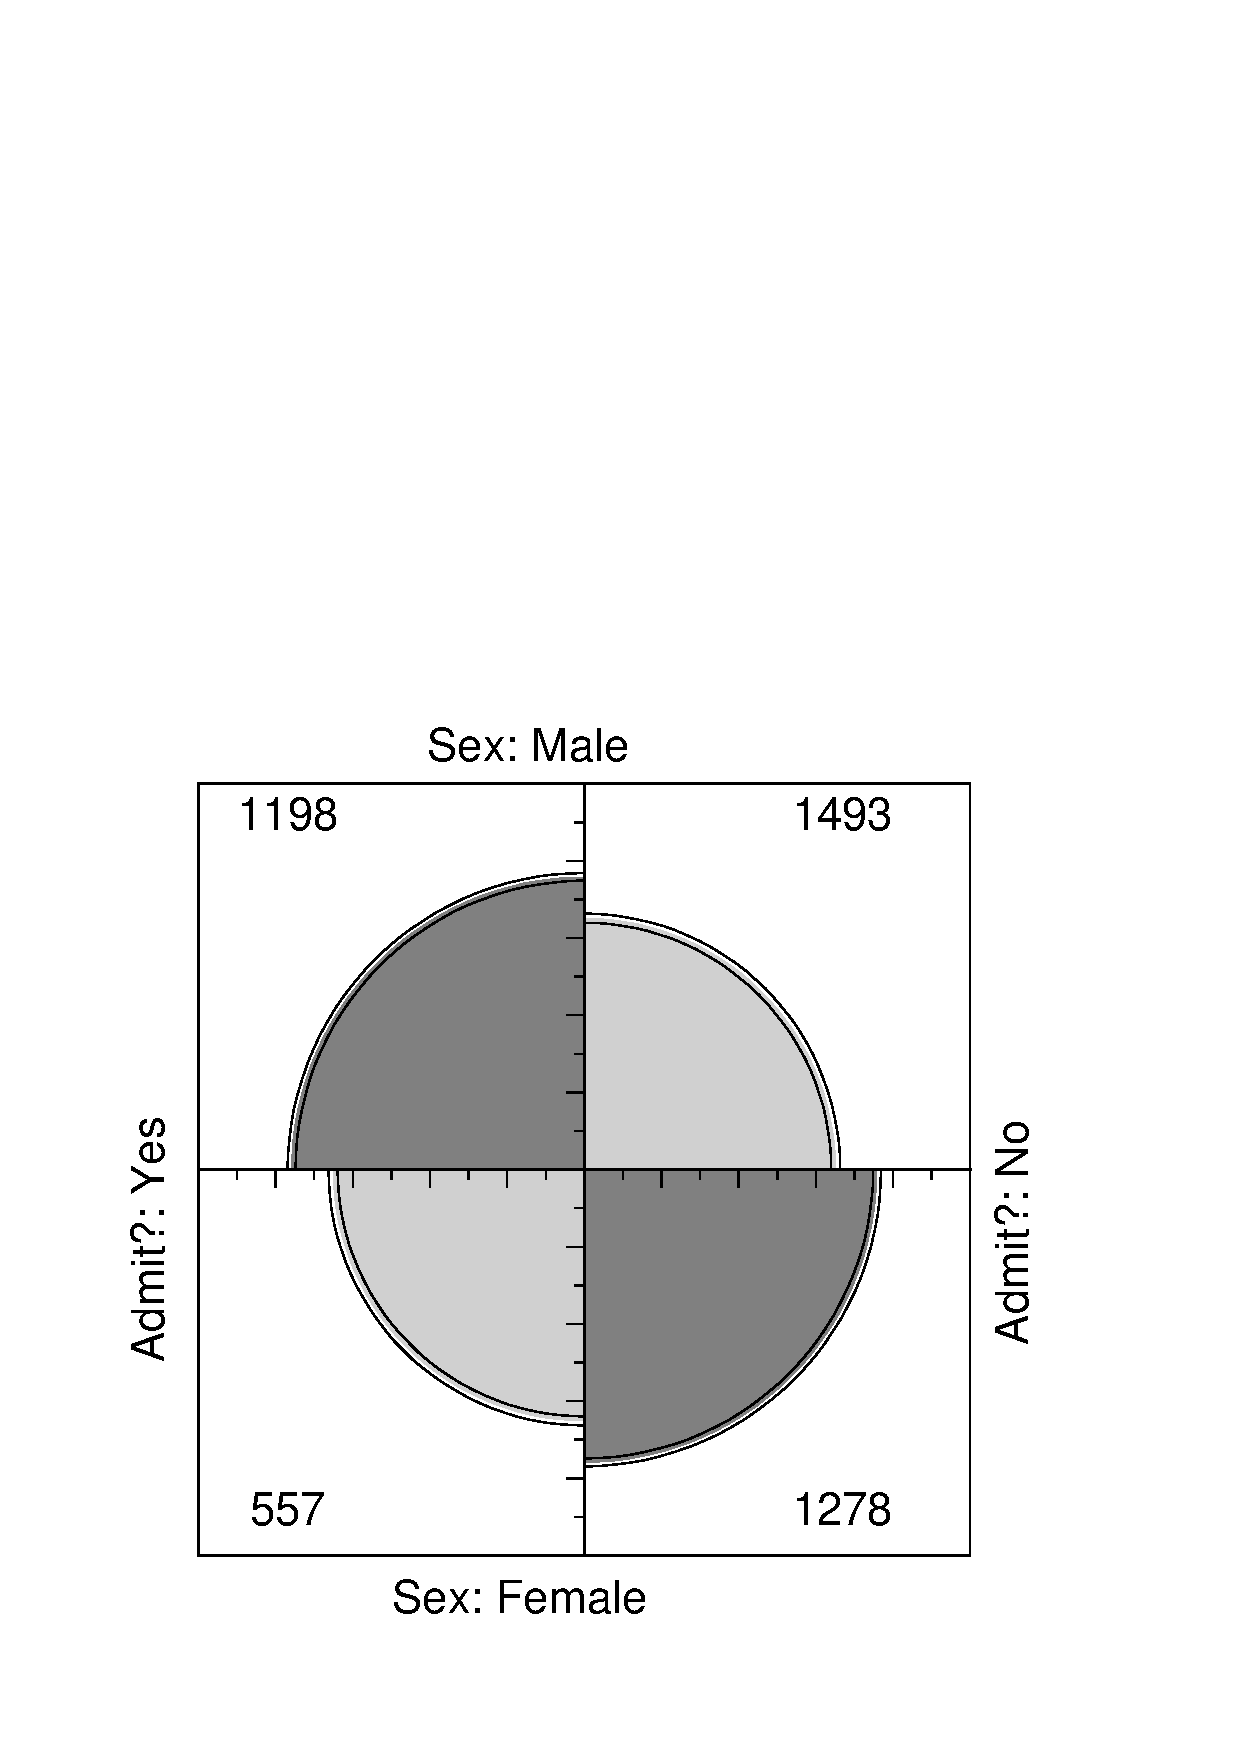
\includegraphics[scale=.6]{ch3/fig/fourfold13}
  \caption[Fourfold display for Berkeley admission data, genders and admission equated]{Fourfold display for Berkeley admission data, genders and admission equated%
. The area of each
quadrant shows the frequency, standardized to equate the margins for
sex and admission.  Circular arcs show the limits of a 99\% confidence
interval for the odds ratio.}\label{fig:fourfold13}
\end{figure}


The quadrants in \figref{fig:fourfold13} do not align and
the 99\% confidence rings around each quadrant do not overlap,
indicating that the odds ratio differs significantly from 1---putative
evidence of gender bias.  The very narrow
width of the confidence rings gives a visual indication of the
precision of the data---if we stopped here, we might feel quite confident of
this conclusion.
\end{Example}

\subsection{Confidence rings for odds ratio}
\ixon{fourfold dislplay!confidence rings}
Confidence rings for the fourfold display are computed from a
confidence interval for \(\theta\), whose endpoints can each be
mapped into a \(2 \times  2\) table.  Each such table is then drawn
in the same way as the data.

The interval for \(\theta\) is most easily found by considering the
distribution of \(\hat{\psi}  =  \log  \hat{\theta} \), whose standard
error may be estimated by \eqref{eq:aselogtheta}.  Then an approximate \(1  -  \alpha\) confidence
interval for \(\psi\) is given by
\begin{equation*}
 \hat{\psi} \,\pm\,  \hat{s} ( \hat{\psi} )  \:
z_{ 1 - \alpha  / 2 } =  \{ \hat{\psi}_l , \,  \hat{\psi}_u \} 
 \comma
\end{equation*}
as described in \secref{sec:twoway-twobytwo}.
The
corresponding limits for the odds ratio \(\theta\) are 
\(\{ \exp ( \hat{\psi}_l ) , \,  \exp ( \hat{\psi}_u ) \}\).  For the data
shown in \figref{fig:fourfold13}, 
\(\hat{\psi}  =  \log \,  \hat{\theta} =  .6104\), 
and \(\hat{s}  ( \hat{\psi} )  =  0.0639\), so the 99\%,
limits for \(\theta\) are \(\{ 1.5617, \,  2.1704 \}\).

Now consider how to find a \(2 \times  2\) table whose frequencies
correspond to the odds ratios at the limits of the confidence
interval.  A table standardized to equal row and column margins can
be represented by the \(2 \times  2\) matrix with entries
\begin{equation*}
 \left[
  \begin{array}{cc}
   p & (1-p) \\
  (1-p) & p
  \end{array}
 \right]
 \comma
\end{equation*}
whose odds ratio is \(\theta  =  p^2 /  ( 1  -  p)^2\).  
Solving for $p$ gives \(p  =  \sqrt \theta /  ( 1  +  \sqrt \theta )\).  The
corresponding frequencies can then be found by adjusting the
standardized table to have the same row and column margins as the
data. The results of these computations which generate the confidence
rings in \figref{fig:fourfold13} are shown in \tabref{tab:berkodds}.

\begin{table}[htb]
\caption{Odds ratios and equivalent tables for confidence rings.}\label{tab:berkodds}
 \begin{center}
\begin{tabular}{lr|rr|rr}
\hline
   &      Odds    & \multicolumn{2}{c|}{Standardized} \\
   &      Ratio   & \multicolumn{2}{c|}{Table}   &  \multicolumn{2}{c}{Frequencies} \\
\hline
Lower &   1.562   &    0.555 & 0.445   &  1157.2 &  1533.8 \\
limit &           &    0.445 & 0.555   &   597.8 &  1237.2 \\[2ex]

Data  &   1.841   &    0.576 & 0.424   &  1198.0 &  1493.0 \\
      &           &    0.424 & 0.576   &   557.0 &  1278.0 \\[2ex]

Upper &   2.170   &    0.596 & 0.404   &  1237.8 &  1453.2 \\
limit &           &    0.404 & 0.596   &   517.2 &  1317.8 \\
\hline
\end{tabular}
\end{center}
\end{table}
\ixoff{fourfold dislplay!confidence rings}

\subsection{The \sasprog{FOURFOLD}}
Fourfold displays have been implemented in \IML{}.
The program is described in detail in an article in
\emph{Observations}
\citep{Friendly:94c}, and is listed and documented in
\macref{mac:fourfold}.

\texttt{fourfold} is a \IML{} module which is called as follows:
\begin{listing}
run fourfold(dim, table, vnames, lnames);
\end{listing}
where \texttt{table} is the $2 \times 2$ (or $2 \times 2 \times k$) frequency table whose dimensions are given by \texttt{dim};
\texttt{vnames} is a character vector containing the names of the table
variables, and
\texttt{lnames} is a character matrix of the category levels.
A variety of options for standardization, shading patterns and colors,
confidence rings, etc.\ are controlled by global variables,
described in \macref{mac:fourfold}.

To use the program, \texttt{\%include} the \sasprog{FOURFOLD}
within a \PROC{IML} step.  Then
enter the observed frequencies in an array \texttt{table},
and create a character vector \texttt{vnames} containing
the row and column variable names, and a two-row
character matrix \texttt{lnames} containing the
category labels.


For example, the plots in \figref{fig:fourfold11} and \figref{fig:fourfold13}
are produced by the statements below.
\begin{listing}
goptions hsize=7in vsize=7in;     *-- make plot square;

filename fourfold  \emph{'path/to/fourfold.sas'};
proc iml;
   %include fourfold;

   *-- Berkeley Admissions data;
   dim = \{2 2\};
   vnames = \{"Admit?" "Sex"\};
   lnames = \{"Yes" "No",
             "Male"  "Female"\};

          /* Admit Not */
   table = \{1198   1493,
             557   1278\};

   patterns=\{solid solid\};
   colors=\{grayd0 gray80\};

   std='MAX';               /* \figref{fig:fourfold11} */
   run fourfold(dim, table, vnames, lnames);

   std='MARG';              /* \figref{fig:fourfold13} */
   run fourfold(dim, table, vnames, lnames);
quit;
\end{listing}
The global variable \texttt{std} determines the way the table is
standardized.
\texttt{std='MAX'} scales the frequencies so that the largest value
is 100; \texttt{std='MARG'} is used to equate the marginal frequencies
for the row variable, the column variable, or both (the default).
The variable(s) equated are controlled by the global \texttt{config}
variable.  For example, to equate the second variable, as in \figref{fig:fourfold12},
you would specify \texttt{config=\{2\}}:
\begin{listing}
   std='MARG';
   config=\{2\};             /* \figref{fig:fourfold12} (equate gender) */
   run fourfold(dim, table, vnames, lnames);
\end{listing}

\subsection{Stratified analysis for $2 \times 2 \times k$ tables}\label{sec:twoway-fourstrat}
In a \(2 \times  2 \times  k\)
table, the last dimension often corresponds to ``strata'' or
populations, and it is typically of interest to see if the
association between the first two variables is homogeneous across
strata.  For such tables, simply make one fourfold panel for each
stratum.  The standardization of marginal frequencies is designed to
allow easy visual comparison of the pattern of association
when the marginal frequencies vary across two
or more populations

The admissions data shown in
\figref{fig:fourfold11}--\figref{fig:fourfold13} were actually obtained
from six departments ---the six largest at Berkeley
\citep{Bickel-etal:75}.
To determine the source of the apparent sex
bias in favor of males, we make a new plot, \figref{fig:pie2x2b},
stratified by department.
\ixd{Berkeley admissions}

Surprisingly, \figref{fig:pie2x2b} shows that, for five of the
six departments, the odds of admission is approximately the same for
both men and women applicants.  Department A appears to differs from
the others, with women approximately 2.86 (\(=  ( 313/19 )  /
(512/89)\)) times as likely to gain admission.  This appearance is
confirmed by the confidence rings, which in \figref{fig:pie2x2b}
are joint 99\% intervals for \(\theta_c ,  \,  c = 1, \dots ,
k\).

\begin{figure}[htb]
  \centering
  \includegraphics[scale=.8]{ch3/fig/pie2x2b}
  \caption[Fourfold display of Berkeley
admissions, by department]{Fourfold display of Berkeley
admissions, by department.  In each panel the confidence rings for
adjacent quadrants overlap if the odds ratio for admission and sex
does not differ significantly from 1.  The data in each panel have
been standardized as in \figref{fig:fourfold13}.}\label{fig:pie2x2b}
\end{figure}

This result, which contradicts the display for the aggregate data in
\figref{fig:fourfold13}, is a nice example of
\emph{Simpson's paradox}%
\footnote{Simpson's paradox \citep{Simpson:51} occurs in a three-way
table, $[A, B, C]$, when the marginal association between two variables,
$A, B$ collapsing over $C$ differs in \emph{direction} from the partial
association $A, B | C= c_k$ at the separate levels of $C$.
Strictly speaking, Simpson's paradox would require that for all
departments separately the odds ratio $\theta_k < 1$
(which occurs for Departments A, B, D, and F in \figref{fig:pie2x2b})
while in the aggregate data $\theta > 1$.
},
and illustrates clearly why an overall analysis of a three- (or higher-)
way table can be misleading.
\ix{Simpson's paradox}
The resolution of this contradiction can be found in the large
differences in admission rates among departments.  Men and women
apply to different departments differentially, and in these data
women happen to apply in larger numbers to departments that have a low
acceptance rate.  The aggregate results are misleading because they
falsely assume men and women are equally likely to apply in each
field.\footnote{This explanation ignores the possibility of structural bias
against women, e.g.,\ lack of resources allocated to departments that
attract women applicants.}

\begin{changebar}
Some final enhancements
of the fourfold display are
 shown in \figref{fig:pie2x2b2}.
Here (a) small tick marks are drawn to show the direction of association
(positive residuals)
and (b) the
\end{changebar} 
intensity of the shading colors is varied to distinguish
those strata for which the odds ratio differs significantly from 1
at $\alpha = .01$.%
\footnote{The \sasprog{FOURFOLD} allows these tests to be done either
individually or jointly (using a Bonferroni adjustment).}

\begin{figure}[htb]
  \centering
  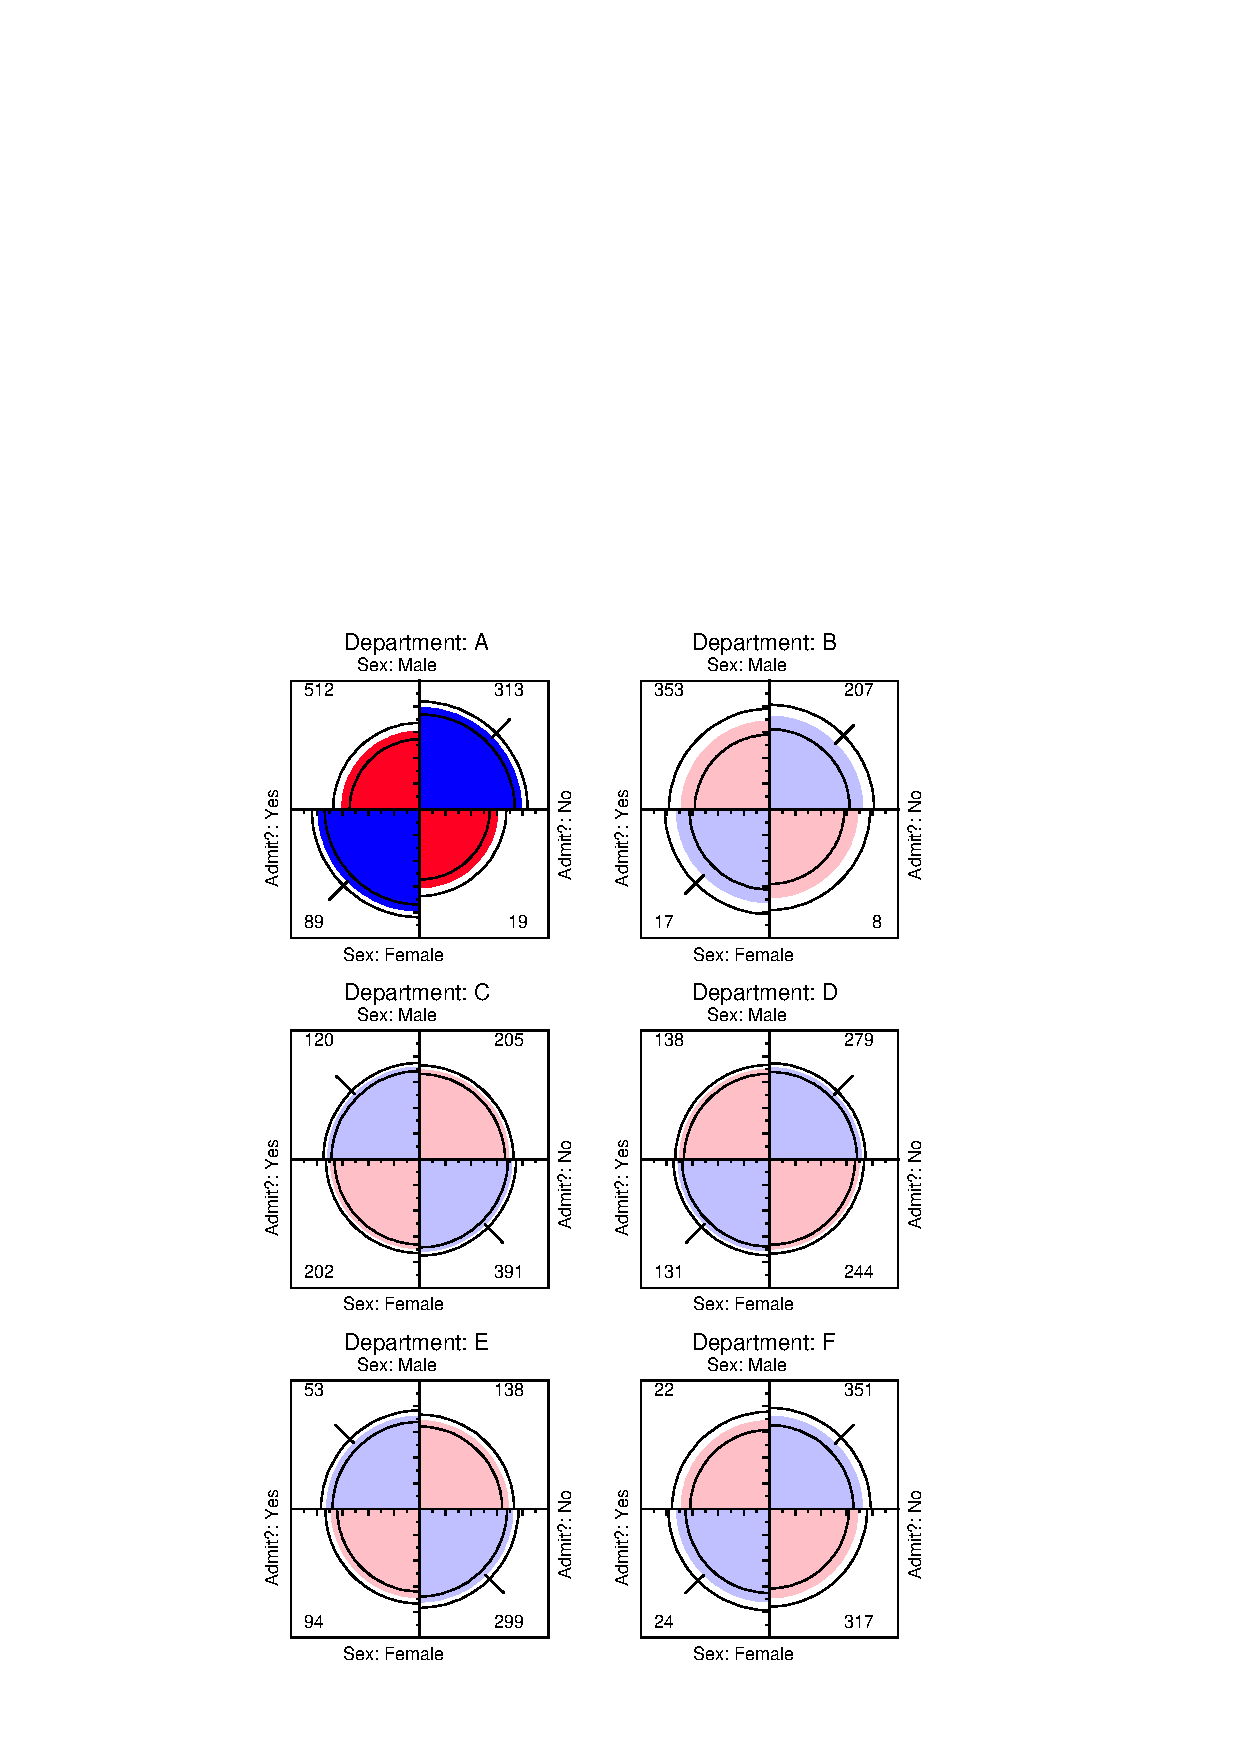
\includegraphics[scale=.8]{ch3/fig/pie2x2b2}
  \caption[Fourfold display of Berkeley
admissions, by department, enhanced]{Fourfold display of Berkeley
admissions, by department, enhanced.  Each panel is shaded
according to whether or not the odds ratio for admission and sex
differs significantly from 1.}\label{fig:pie2x2b2}
\end{figure}

\subsubsection{Visualization principles}
An important principle in the display of large, complex \Dsets\
is \boldital{controlled comparison}---we want to make comparisons
against a clear standard, with
other things held constant.
The fourfold display
differs from a pie chart in that it holds the
angles of the segments constant and varies the radius.
An important consequence is that we can quite easily compare a
series of fourfold displays for different strata, since corresponding
cells of the table are always in the same position.
As a result, an array of fourfold displays serve the goals of comparison and
detection better than an array of pie charts.
Moreover, it allows the observed frequencies to be standardized
by equating either the row or column totals, while preserving
the odds ratio.
In \figref{fig:pie2x2b}, for example,
the proportion of men and women, and the proportion
of accepted applicants were equated visually in each department.
This provides a clear standard which
also greatly facilitates controlled comparison.

Another principle is \boldital{visual impact}---we want the important
features
of the display to be easily distinguished from the less important
\citep{Tukey:93}.
\figref{fig:pie2x2b2} distinguishes the one department for which
the odds ratio differs significantly from 1 by shading intensity,
even though the same information can be found by inspection of the
confidence rings.

\begin{Example}[wheeze1]{Breathlessness and wheeze in coal miners}
The various ways of standardizing a collection of $2 \times 2$ tables
allows visualizing relations with different factors
(row percentages, column percentages, strata totals) controlled.
Different graphs can speak more eloquently to different questions.

\citet[Table 7.11]{Agresti:90} cites data from
\citet{AshfordSnowden:70} on the association between
two pulmonary conditions, breathlessness and wheeze, in a large sample of coal miners.
The miners are classified into age groups, and the question treated
by Agresti is whether the association between these two symptoms
is homogeneous over age.%
\footnote{A ninth group, aged 20-24 has been omitted from these
analyses.}
This question is addressed by displaying the odds ratio
in the $2 \times 2$ tables with the margins of breathlessness
and wheeze equated (i.e., with the default \pname{std='MARG';} option),
which gives the graph shown in \figref{fig:pie2x2wh1}.
Although the panels for all age groups show an overwhelmingly
positive association between these two symptoms, one can also
see that the strength of this association declines with increasing
age.

Note that the pattern of change over age is somewhat subtle
compared to the dominant positive association within each
panel.
When the goal is to display how the odds ratio varies with
a quantitative factor such as age, it is often better to simply
plot the odds ratio directly, as shown in \figref{fig:pie2x2wh2}.

The \sasprog{FOURFOLD} also provides the relevant test statistics,
shown in \outref{out:pie2x2wh}.
The test of whether the association is the same over age
is a test of the \loglin{} model
[BW][BA][WA] of no three-way association among the
variables Breathlessness, Wheeze and Age,
which is soundly rejected,
$G^2 (7) = 26.13$.

\begin{figure}[htb]
  \centering
  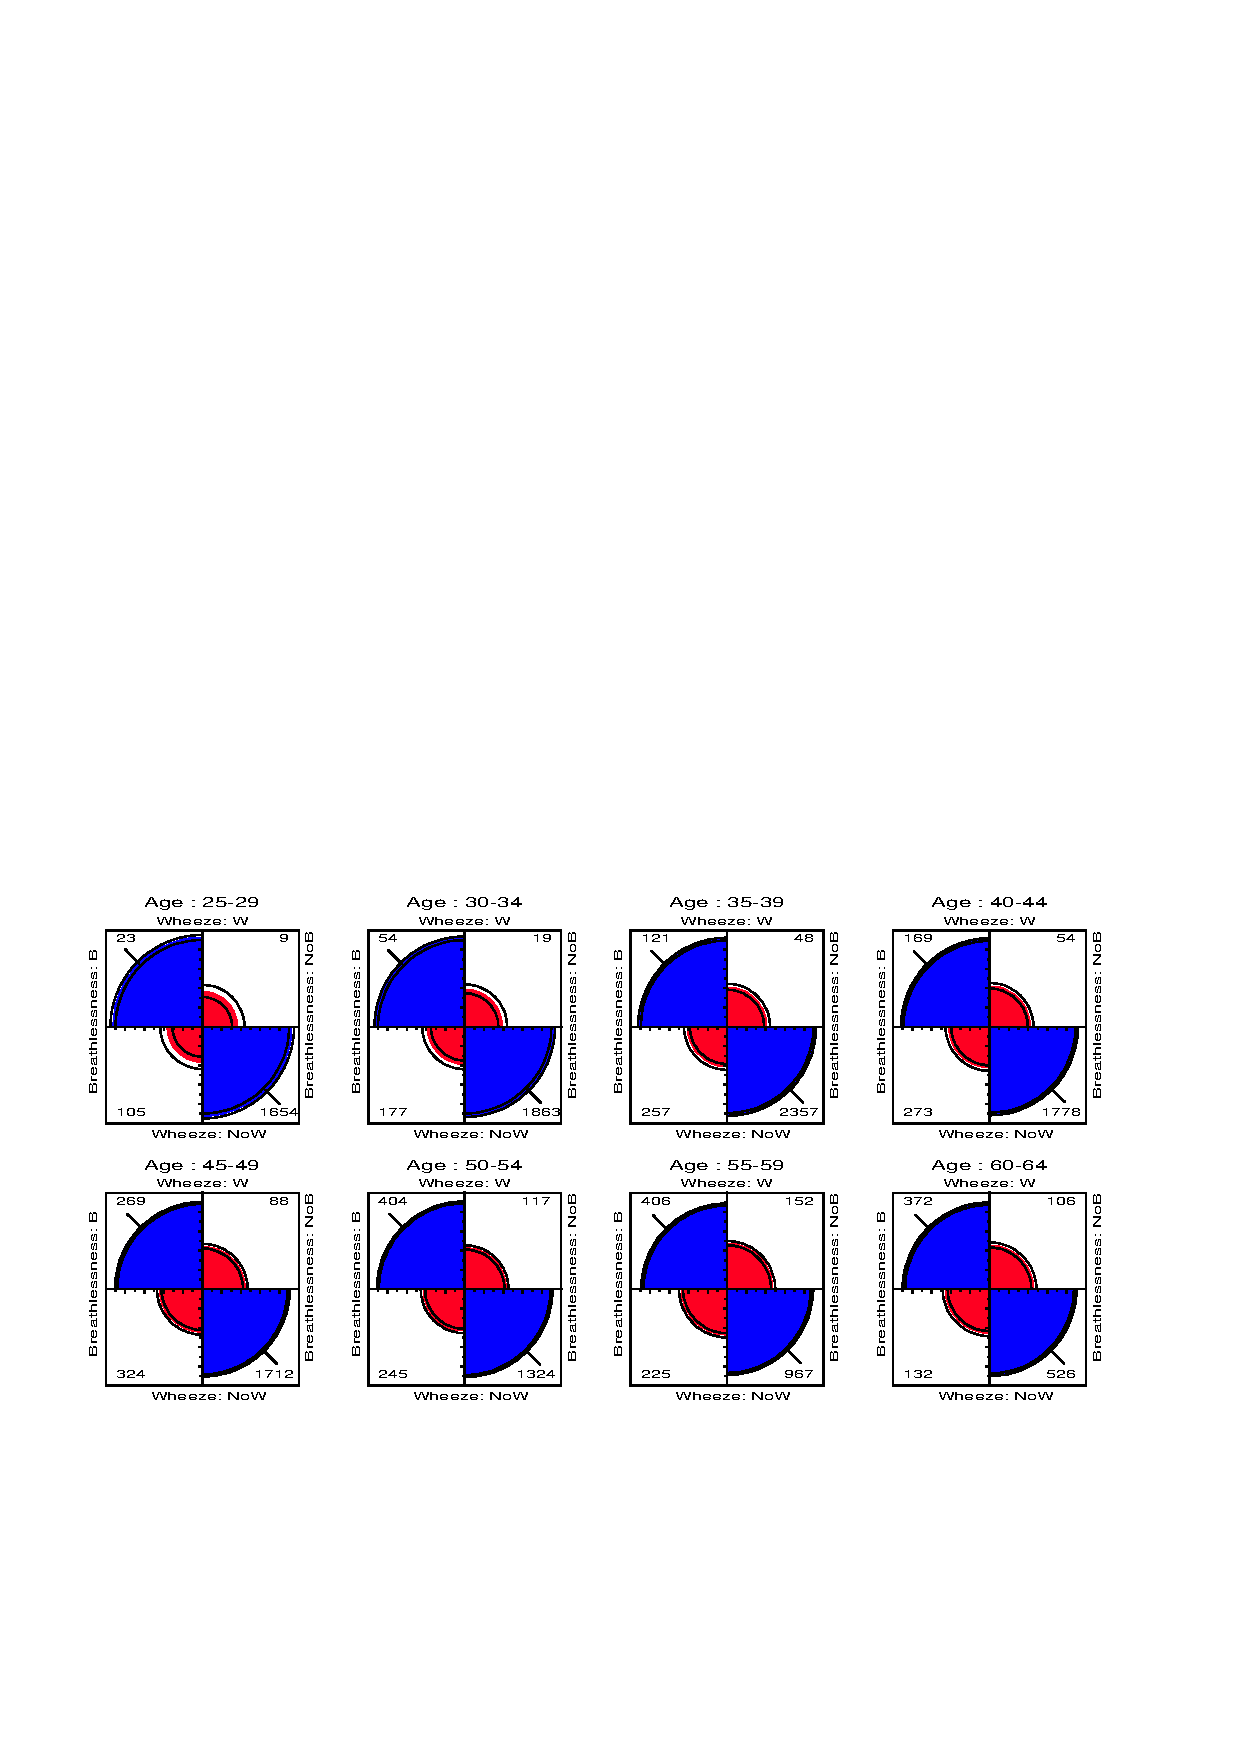
\includegraphics[scale=.8,clip]{ch3/fig/pie2x2wh1}
  \caption[Fourfold display for coal miners data, both margins equated]{Fourfold display for coal miners data, both margins equated.}\label{fig:pie2x2wh1}
\end{figure}
%
\begin{Output}
\caption{Odds ratios and tests of homogeneity of association for coal miners data}\label{out:pie2x2wh}
\small
\verbatiminput{ch3/out/pie2x2wh.out}
\end{Output}

\begin{figure}[htb]
  \centering
  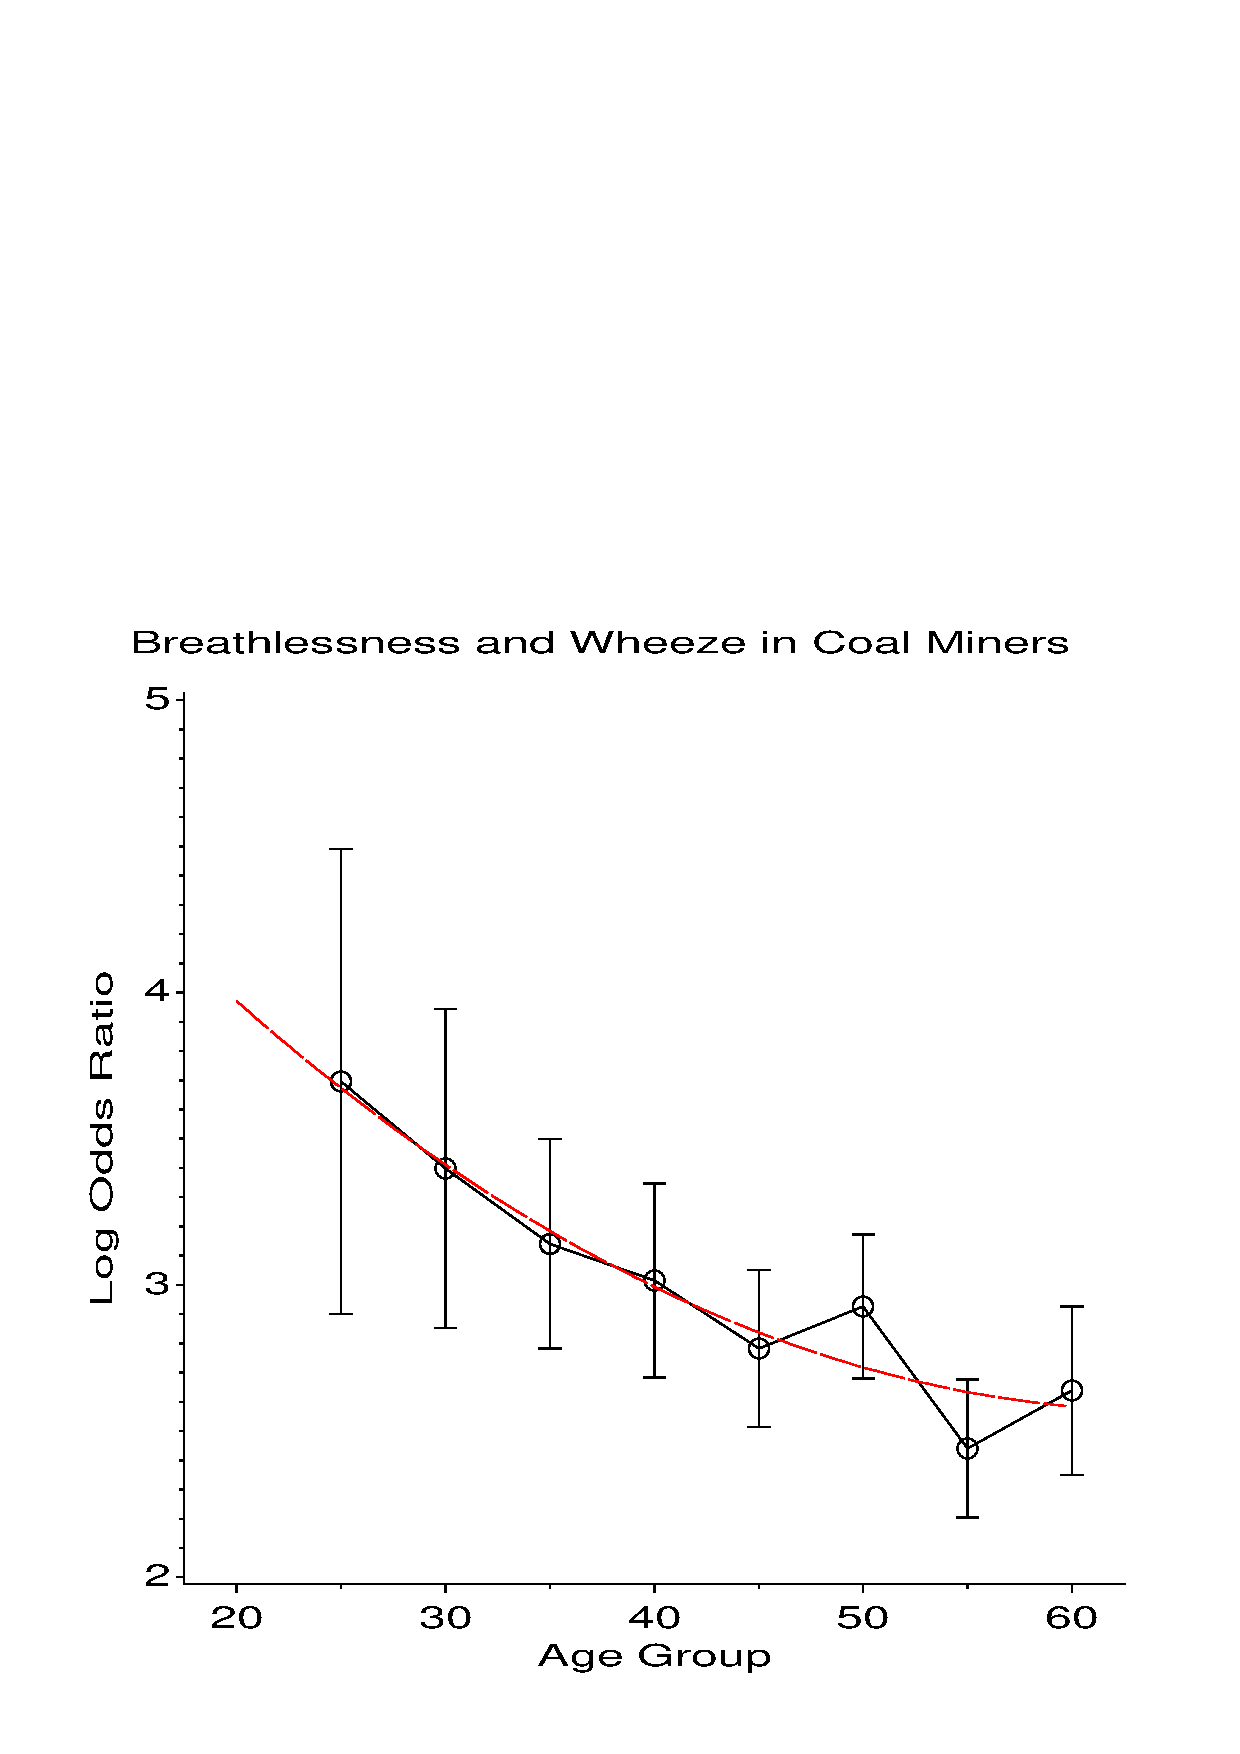
\includegraphics[scale=.6]{ch3/fig/pie2x2wh2}
  \caption[Breathlessness and wheeze in coal miners, odds ratios]{Breathlessness and wheeze in coal miners, log odds plot.  The smooth curve is a quadratic fit.
  Vertical bars give individual 95\% confidence intervals.}\label{fig:pie2x2wh2}
\end{figure}

A more poignant question, however, concerns the prevalence of these
two respiratory symptoms among miners and how these change over age.
The answer is concealed in \figref{fig:pie2x2wh1}, since the
proportion of miners with each symptom are equated in each age group.
This question can be addressed by standardizing the frequencies
to equate the numbers in each stratum (\texttt{std='MAX';}),
which gives the graph shown in \figref{fig:pie2x2wh3}.
If one regards age as reflecting number of years spent working
in coal mines,
this figure shows the sad result of such employment:
the relative frequency of miners with both symptoms steadily
increasing over age.
We return to these data in \exref{ex:ashford},
where we consider a variety of specific
logit models for the prevalence of each symptom
simultaneously with models for their log odds ratio.
\begin{figure}[htb]
  \centering
  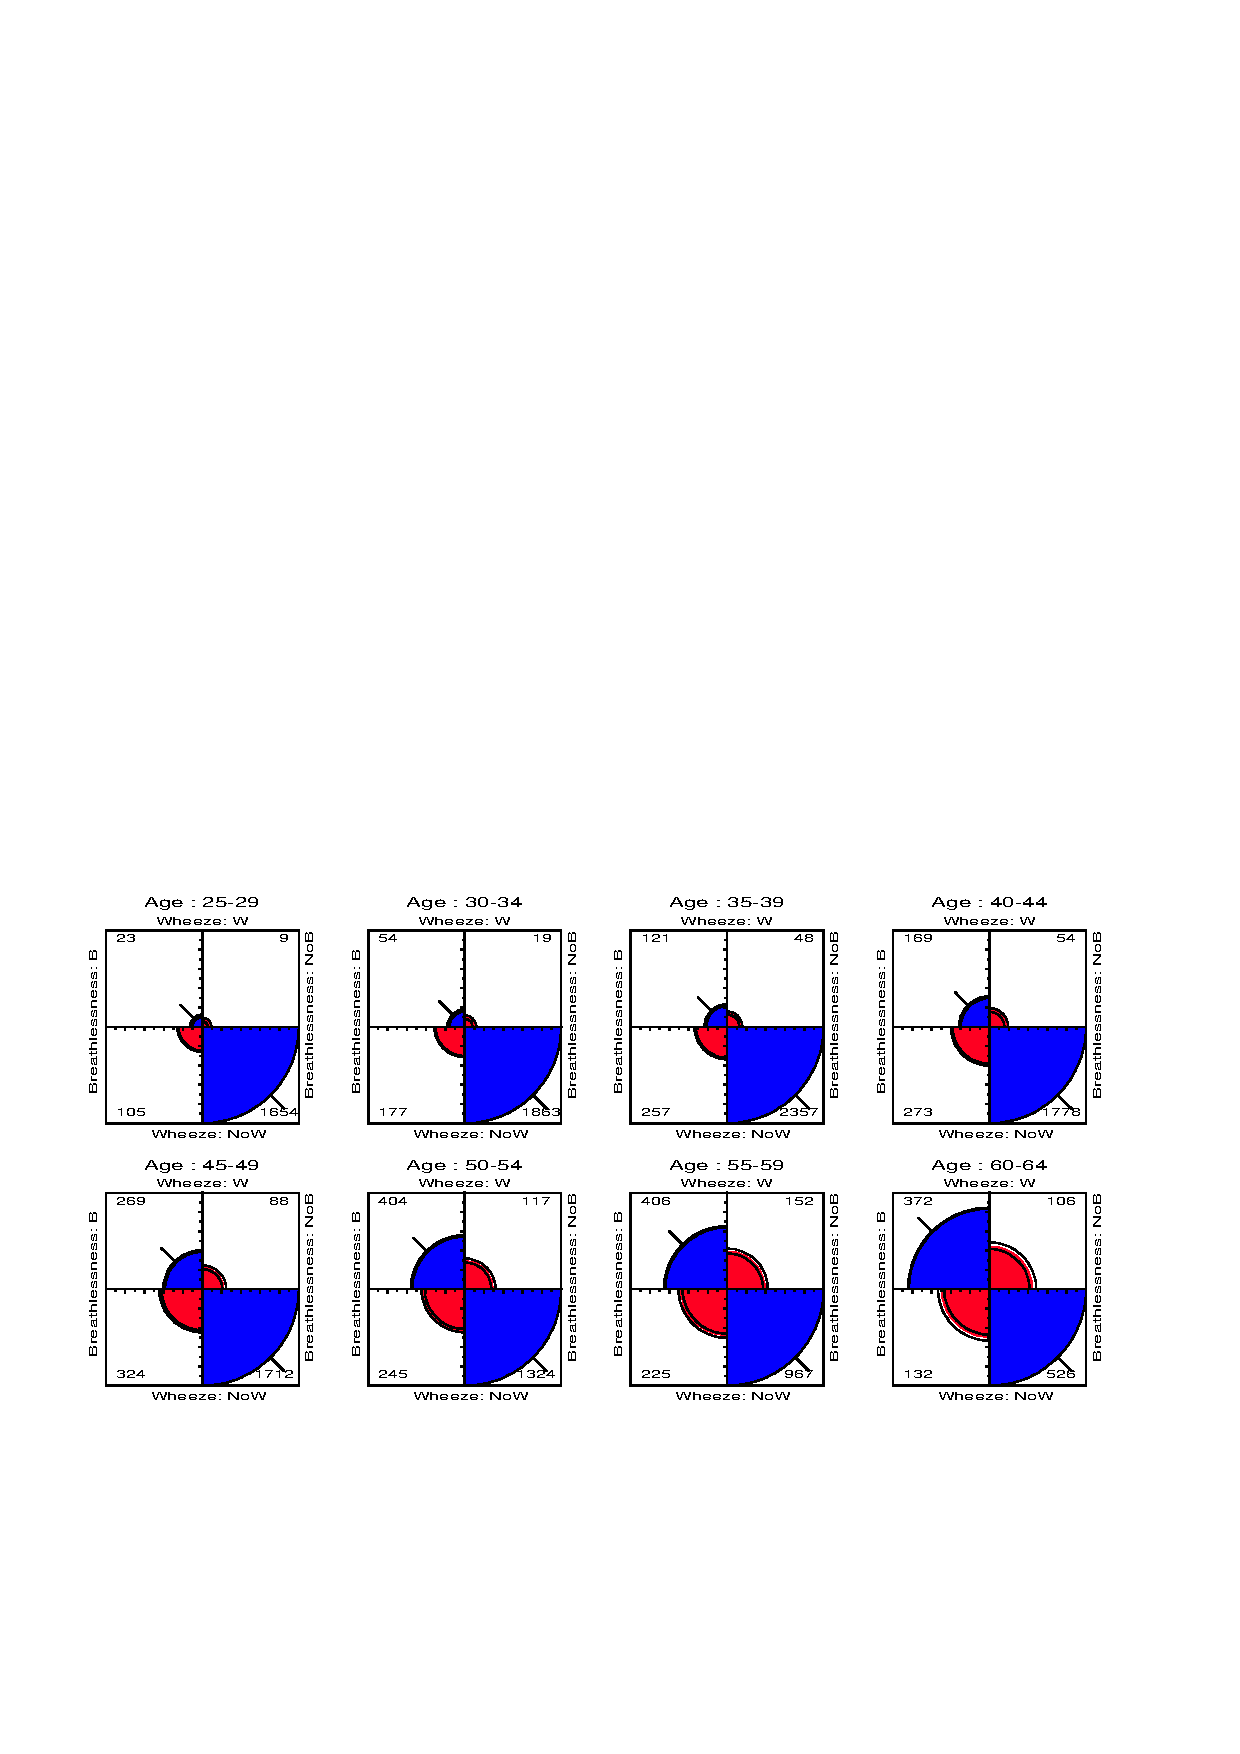
\includegraphics[scale=.8,clip]{ch3/fig/pie2x2wh3}
  \caption[Fourfold display for coal miners data, strata equated]{Fourfold display for coal miners data, strata equated.}\label{fig:pie2x2wh3}
\end{figure}
\end{Example}

%\begin{changebar}
%\begin{Example}[toxaemia0]{Toxaemic symptoms in pregnancy}
In \secref{sec:loglin-multiv}, we examine multivariate models
for two or more categorical responses.
\exref{ex:toxaemia} presents an analysis of data from
\citet{Brown-etal:83}
on the occurrence of two
signs of toxaemia (hypertension and protein urea)
among 13,384 expectant mothers in Bradford, England in their first pregnancy.
The mothers are classified by social class (1--5), and by the
number of cigarettes smoked per day (0, 1--19, or $20+$).

The models presented later describe how both the marginal distributions
of the responses, \emph{and} their association, vary with explanatory variables.
Here, we preview those data with a fourfold display focused on just
the association (odds ratio) between the two binary
response variables, Hypertension and Urea.


%% one figure
\begin{figure}[htb]
  \centering
  \includegraphics[width=\linewidth,clip]{ch3/fig/4ftox.eps}
  \caption[Fourfold display for toxaemia data]{Fourfold display for toxaemia data.  The level of mother's smoking increases from top to bottom;
  mother's social class increases from left to right}%
  \label{fig:4ftox}
\end{figure}

\figref{fig:4ftox} shows the fourfold displays for the 15 combinations
of mother's social class and smoking, with non-smokers in the top row,
and heaviest smokers in the bottom row.
We see that, with one exception (a cell with small total frequency),
the association between presence of hypertension and urea
is positive, and roughly of the same magnitude over the categories
of class, particularly for non- and moderate-smokers.
In \exref{ex:toxaemia} we plot the log odds ratio directly (\figref{fig:tox13}), as well as the log odds for prevalence
of these two symptoms.
\end{Example}

%\end{changebar}
\ixoff{fourfold display}
